\documentclass[tikz,border=12pt]{standalone}
\usepackage[T1]{fontenc}
\usepackage{mathpazo}
\usepackage{amsmath,amssymb}
\usetikzlibrary{arrows.meta, positioning, calc, fit, decorations.pathreplacing, patterns}

\definecolor{stblue}{HTML}{7B97AD}
\definecolor{rwgold}{HTML}{B8995E}
\definecolor{sage}{HTML}{7A9A7E}
\definecolor{dkbrown}{HTML}{3D3530}
\definecolor{wmgray}{HTML}{7B7067}
\definecolor{cream}{HTML}{F9F6F0}
\definecolor{border}{HTML}{D4C9B8}
\definecolor{terracotta}{HTML}{C47A6A}
\definecolor{lavender}{HTML}{907EA0}

\begin{document}
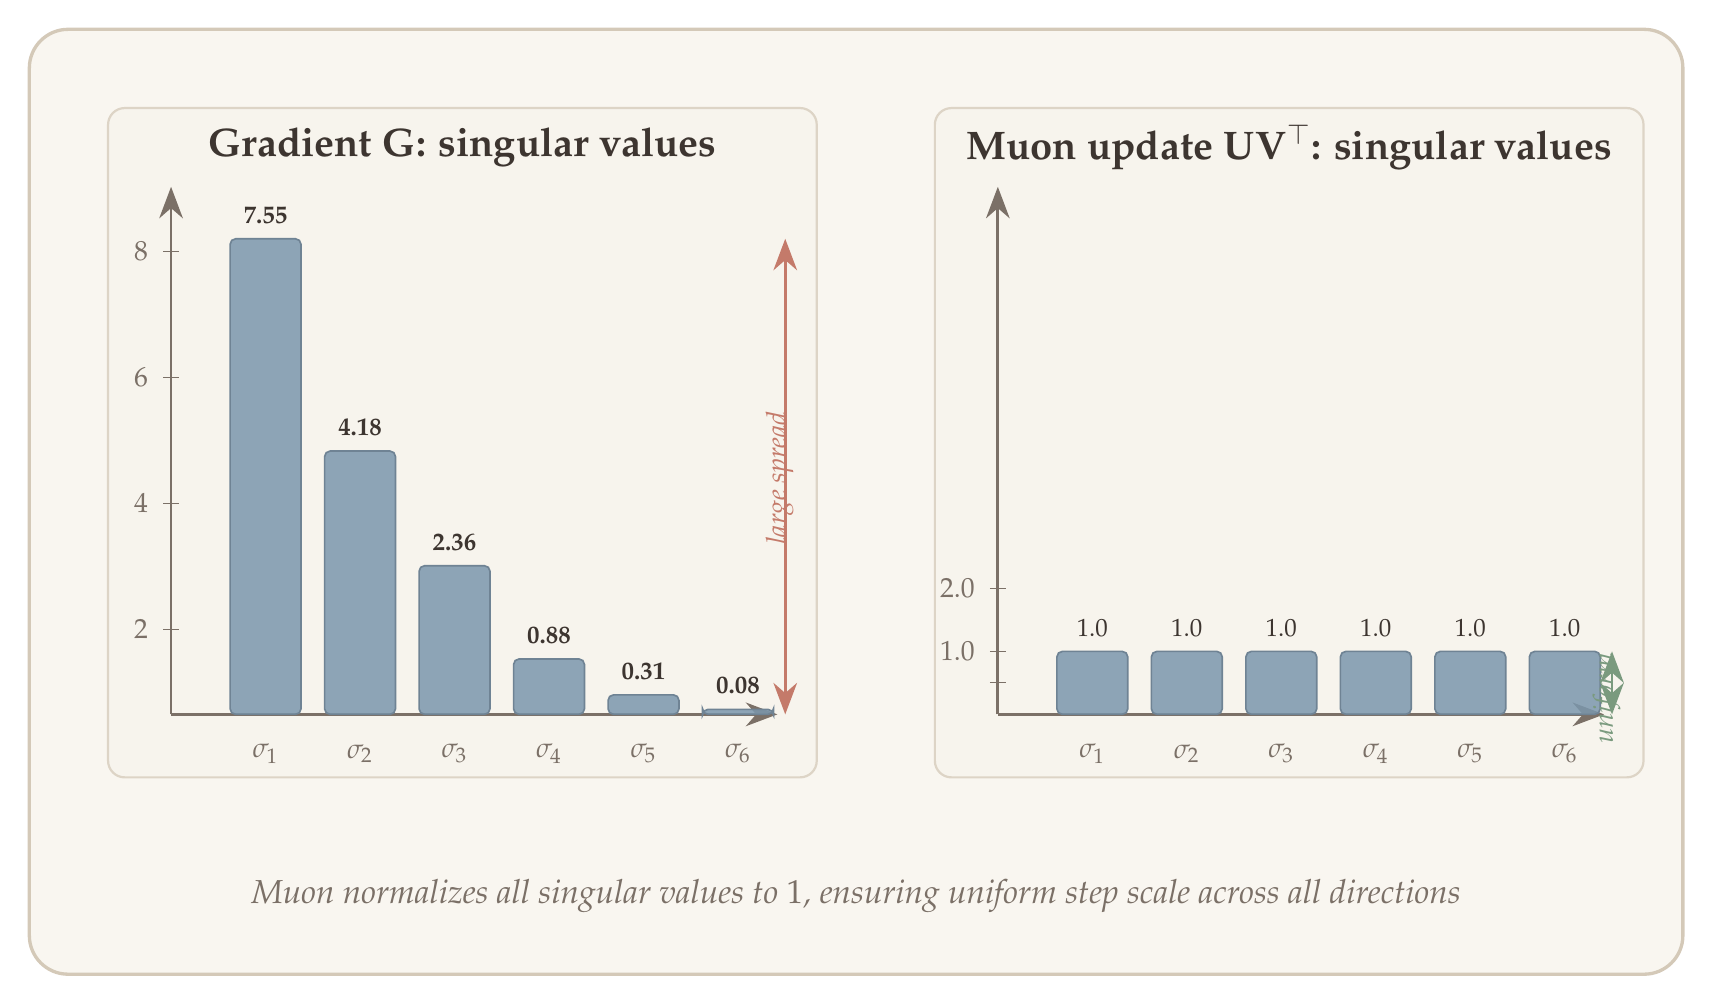
\begin{tikzpicture}[>={Stealth[length=4mm, width=3mm]}, line width=1.5pt]

% Background
\fill[cream, rounded corners=14pt] (-0.5,-2.5) rectangle (20.5,9.5);
\draw[border, line width=1.2pt, rounded corners=14pt] (-0.5,-2.5) rectangle (20.5,9.5);

% ============================================================
% Left panel: Gradient singular values
% ============================================================
\def\panelLx{0.5}
\def\panelLy{0.0}

% Panel background
\fill[cream!95!border, rounded corners=6pt] (\panelLx,\panelLy) rectangle ($({\panelLx+9.0},{\panelLy+8.5})$);
\draw[border!80, line width=0.8pt, rounded corners=6pt] (\panelLx,\panelLy) rectangle ($({\panelLx+9.0},{\panelLy+8.5})$);

% Panel title
\node[text=dkbrown, font=\Large\bfseries] at ($({\panelLx+4.5},{\panelLy+8.0})$) {Gradient $\mathbf{G}$: singular values};

% Axes
\draw[wmgray, ->, line width=1pt] ($({\panelLx+0.8},{\panelLy+0.8})$) -- ($({\panelLx+8.5},{\panelLy+0.8})$);
\draw[wmgray, ->, line width=1pt] ($({\panelLx+0.8},{\panelLy+0.8})$) -- ($({\panelLx+0.8},{\panelLy+7.5})$);

% Y-axis ticks and labels
\foreach \val/\ypos in {2/1.88, 4/3.48, 6/5.08, 8/6.68} {
  \draw[wmgray, line width=0.4pt] ($({\panelLx+0.7},{\panelLy+\ypos})$) -- ($({\panelLx+0.9},{\panelLy+\ypos})$);
  \node[text=wmgray, font=\normalsize, anchor=east] at ($({\panelLx+0.65},{\panelLy+\ypos})$) {$\val$};
}

% Bar width and spacing
% Bars: sigma_1=7.55, sigma_2=4.18, sigma_3=2.36, sigma_4=0.88, sigma_5=0.31, sigma_6=0.08
% Scale: height = value * 0.8 (so 8 -> 6.4 units)
\def\bscale{0.8}
\def\bwidth{0.9}
\def\bbase{0.8} % y-base

% Bar positions (x-centers)
\foreach \idx/\val/\xc in {1/7.55/2.0, 2/4.18/3.2, 3/2.36/4.4, 4/0.88/5.6, 5/0.31/6.8, 6/0.08/8.0} {
  \pgfmathsetmacro{\bh}{\val*\bscale}
  \fill[stblue, opacity=0.85, rounded corners=2pt]
    ($({\panelLx+\xc-\bwidth/2},{\panelLy+\bbase})$)
    rectangle
    ($({\panelLx+\xc+\bwidth/2},{\panelLy+\bbase+\bh})$);
  \draw[stblue!80!dkbrown, line width=0.6pt, rounded corners=2pt]
    ($({\panelLx+\xc-\bwidth/2},{\panelLy+\bbase})$)
    rectangle
    ($({\panelLx+\xc+\bwidth/2},{\panelLy+\bbase+\bh})$);
  % Value label above bar
  \node[text=dkbrown, font=\small\bfseries] at ($({\panelLx+\xc},{\panelLy+\bbase+\bh+0.3})$) {\val};
  % X-axis label
  \node[text=wmgray, font=\normalsize] at ($({\panelLx+\xc},{\panelLy+0.3})$) {$\sigma_\idx$};
}

% Annotation: spread
\draw[terracotta, <->, line width=1pt] ($({\panelLx+8.6},{\panelLy+\bbase})$) -- ($({\panelLx+8.6},{\panelLy+\bbase+7.55*\bscale})$);
\node[text=terracotta, font=\normalsize\itshape, rotate=90, anchor=south] at ($({\panelLx+8.85},{\panelLy+\bbase+3.0})$) {large spread};

% ============================================================
% Right panel: Muon update singular values
% ============================================================
\def\panelRx{11.0}
\def\panelRy{0.0}

% Panel background
\fill[cream!95!border, rounded corners=6pt] (\panelRx,\panelRy) rectangle ($({\panelRx+9.0},{\panelRy+8.5})$);
\draw[border!80, line width=0.8pt, rounded corners=6pt] (\panelRx,\panelRy) rectangle ($({\panelRx+9.0},{\panelRy+8.5})$);

% Panel title
\node[text=dkbrown, font=\Large\bfseries] at ($({\panelRx+4.5},{\panelRy+8.0})$) {Muon update $\mathbf{U}\mathbf{V}^\top$: singular values};

% Axes
\draw[wmgray, ->, line width=1pt] ($({\panelRx+0.8},{\panelRy+0.8})$) -- ($({\panelRx+8.5},{\panelRy+0.8})$);
\draw[wmgray, ->, line width=1pt] ($({\panelRx+0.8},{\panelRy+0.8})$) -- ($({\panelRx+0.8},{\panelRy+7.5})$);

% Y-axis ticks
\foreach \val/\ypos in {0.5/1.2, 1.0/1.6, 2/2.4} {
  \draw[wmgray, line width=0.4pt] ($({\panelRx+0.7},{\panelRy+\ypos})$) -- ($({\panelRx+0.9},{\panelRy+\ypos})$);
}
\node[text=wmgray, font=\normalsize, anchor=east] at ($({\panelRx+0.65},{\panelRy+1.6})$) {$1.0$};
\node[text=wmgray, font=\normalsize, anchor=east] at ($({\panelRx+0.65},{\panelRy+2.4})$) {$2.0$};

% All bars at height 1.0 -> 0.8 units in plot
\foreach \idx/\xc in {1/2.0, 2/3.2, 3/4.4, 4/5.6, 5/6.8, 6/8.0} {
  \fill[stblue, opacity=0.85, rounded corners=2pt]
    ($({\panelRx+\xc-\bwidth/2},{\panelRy+\bbase})$)
    rectangle
    ($({\panelRx+\xc+\bwidth/2},{\panelRy+\bbase+0.8})$);
  \draw[stblue!80!dkbrown, line width=0.6pt, rounded corners=2pt]
    ($({\panelRx+\xc-\bwidth/2},{\panelRy+\bbase})$)
    rectangle
    ($({\panelRx+\xc+\bwidth/2},{\panelRy+\bbase+0.8})$);
  % Value label
  \node[text=dkbrown, font=\small\bfseries] at ($({\panelRx+\xc},{\panelRy+\bbase+1.1})$) {$1.0$};
  % X-axis label
  \node[text=wmgray, font=\normalsize] at ($({\panelRx+\xc},{\panelRy+0.3})$) {$\sigma_\idx$};
}

% Annotation: uniform
\draw[sage, <->, line width=1pt] ($({\panelRx+8.6},{\panelRy+\bbase})$) -- ($({\panelRx+8.6},{\panelRy+\bbase+0.8})$);
\node[text=sage, font=\normalsize\itshape, rotate=90, anchor=south] at ($({\panelRx+8.85},{\panelRy+\bbase+0.2})$) {uniform};

% Bottom annotation
\node[text=wmgray, font=\large\itshape] at (10.0,-1.5) {Muon normalizes all singular values to $1$, ensuring uniform step scale across all directions};

\end{tikzpicture}
\end{document}
